\providecommand{\econtexRoot}{}
\renewcommand{\econtexRoot}{..}
\providecommand{\econtexPaths}{}\renewcommand{\econtexPaths}{\econtexRoot/Resources/econtexPaths}
% The \commands below are required to allow sharing of the same base code via Github between TeXLive on a local machine and Overleaf (which is a proxy for "a standard distribution of LaTeX").  This is an ugly solution to the requirement that custom LaTeX packages be accessible, and that Overleaf prohibits symbolic links
\providecommand{\econtex}{\econtexRoot/Resources/texmf-local/tex/latex/econtex}
\providecommand{\econtexSetup}{\econtexRoot/Resources/texmf-local/tex/latex/econtexSetup}
\providecommand{\econtexShortcuts}{\econtexRoot/Resources/texmf-local/tex/latex/econtexShortcuts}
\providecommand{\econtexBibMake}{\econtexRoot/Resources/texmf-local/tex/latex/econtexBibMake}
\providecommand{\econtexBibStyle}{\econtexRoot/Resources/texmf-local/bibtex/bst/econtex}
\providecommand{\econtexBib}{\econtexRoot/Resources/texmf-local/bibtex/bib/economics}
\providecommand{\notes}{\econtexRoot/Resources/texmf-local/tex/latex/handout}
\providecommand{\handoutSetup}{\econtexRoot/Resources/texmf-local/tex/latex/handoutSetup}
\providecommand{\handoutShortcuts}{\econtexRoot/Resources/texmf-local/tex/latex/handoutShortcuts}
\providecommand{\handoutBibMake}{\econtexRoot/Resources/texmf-local/tex/latex/handoutBibMake}
\providecommand{\handoutBibStyle}{\econtexRoot/Resources/texmf-local/bibtex/bst/handout}

\providecommand{\FigDir}{\econtexRoot/Figures}
\providecommand{\CodeDir}{\econtexRoot/Code}
\providecommand{\DataDir}{\econtexRoot/Data}
\providecommand{\SlideDir}{\econtexRoot/Slides}
\providecommand{\TableDir}{\econtexRoot/Tables}
\providecommand{\ApndxDir}{\econtexRoot/Appendices}

\providecommand{\ResourcesDir}{\econtexRoot/Resources}
\providecommand{\rootFromOut}{..} % Path back to root directory from output-directory
\providecommand{\LaTeXGenerated}{\econtexRoot/LaTeX} % Put generated files in subdirectory
\providecommand{\econtexPaths}{\econtexRoot/Resources/econtexPaths}
\providecommand{\LaTeXInputs}{\econtexRoot/Resources/LaTeXInputs}
\providecommand{\LtxDir}{LaTeX/}
\providecommand{\EqDir}{Equations} % Put generated files in subdirectory
\documentclass[pdflatex]{beamer}
\providecommand{\texname}{ProjectKWK-Slides}% Indicate the keyname for the bibtex entry corresponding to this document
\providecommand{\texnameMaster}{ProjectKWK}% Indicate the keyname for the bibtex entry corresponding to this document
\newif\ifdvi\dvifalse

%\usepackage{optional}
\usepackage{ifthen}%\usepackage{\econtexRoot/ProjectKWK}

% Can't read in ProjectKWK.sty because some packages conflict with Beamer
% So need to redefine everything here

\usepackage{\econtexShortcuts}
\usepackage{natbib,amsmath,amssymb,rotating,subfigure}
\usepackage{verbatim,moreverb,graphicx}
\usepackage{wasysym}
\usepackage{dcolumn}
\usepackage{cancel}

%\providecommand{\LtxDir\EqDir}{\econtexRoot/Equations}
\providecommand{\FigsRaw}{\econtexRoot/Code/Python/Figures}
\providecommand{\CodeDir}{\econtexRoot/Code}
\providecommand{\CalibrationDir}{\econtexRoot/Calibration}
\providecommand{\TableDir}{\econtexRoot/Tables}
\providecommand{\ApndxDir}{\econtexRoot/Appendices}
\providecommand{\Ex}{\mathbb{E}}

%\usepackage{natbib}\newcommand*{\newblock}{}

\mode<presentation>
{
  \usetheme{Warsaw}
  % or ...
  \setbeamercovered{transparent}
}

%\beamerdefaultoverlayspecification{<+->}

%\setbeamertemplate{navigation symbols}{}  % Take away navigation symbols

\usetheme{Warsaw}

\setbeamersize{text margin left=3mm}
\setbeamersize{text margin right=3mm}


%_____________ Opening slide _______________________

\title[Close Elections]{Close Elections, Campaign Contributions, and Financial Deregulation}
\author[Koh]{Kyung Woong Koh}
\institute[JHU]{Johns Hopkins University}
\date[\today]{\today}

\begin{document}\bibliographystyle{\econtexBibStyle}

\begin{frame}[plain]
  \titlepage
\end{frame}


%_____________ 1st section  ____________
\section{Introduction}
\subsection{Motivation}


\begin{frame}
\frametitle{Introduction}

\pause Are legislators in close elections more susceptible to special interests?
\begin{itemize}
	\item Answers within the context of financial deregulation
	\item Igan and Mishra (2014): Looks at legislators being susceptible to special interests of financial industry concerning deregulation of lending practices
	\item New contribution of this paper: Legislators in \textbf{close elections}
\end{itemize}
\end{frame}


\begin{frame}{Key Result}
\pause
Not here yet
\begin{itemize}
\item But will come up soon
\end{itemize}

\end{frame}


\section{Mechanism}
\begin{frame}
\frametitle{Mechanism of Legislators' Vote Switching}

\begin{figure}[ht]
  \centerline{
    \includegraphics[width=0.8\textwidth]{\FigDir/KohFigure1_tikzmake}
  }
    \caption{Two Channels in which Legislators in Close Elections Switch their Votes Toward Financial Deregulation}\label{KohFigure1}
\end{figure}

\end{frame}


\section{Variables}

\begin{frame}
\frametitle{Dependent Variable}

\newsavebox{\DepVar}
\begin{table}
\centering
\caption{Definition of the Main Dependent Variable, Vote Switch towards Deregulation}\label{table:DepVar}
\sbox{\DepVar}{
\begin{tabular}{p{0.25\linewidth} | p{0.25\linewidth} | p{0.25\linewidth}} \hline
\textbf{Value of $S_iBR$}  & Voted for deregulation in Bill $B,R$ & Voted against deregulation in Bill $B,R$ \\ \hline
Voted for deregulation in Bill $B,R-1$ & 0 & 0 \\ \hline
Voted for deregulation in Bill $B,R-1$ & 1 & 0 \\ \hline
\end{tabular}
}
\usebox{\DepVar}
\end{table}

\end{frame}



\section{Regression Strategy}

\begin{frame}
\frametitle{Regression A-1}

Regression A1: Regression with only close election and relevant interaction terms
\begin{align}
    S_{iBR} &= \beta_{1} L_{BR} + \beta_{2} X_{iBR}^{P} + \beta_{3} (L_{BR} \times X_{iBR}^{P} ) \nonumber \\
    &+ \alpha F_{BR} + \gamma T_{BR}+ s_{i} \times t_{c}+ v_{B} \times t_{c}+\mu_{R} \times t_{c}+\varepsilon_{iBR}
\end{align}


\end{frame}


\subsection{The Perfect Foresight Problem}

\begin{frame}
\frametitle{Benchmark: Perfect Foresight Model}

Definitions: \smallskip

\begin{tabular}{llcl}
   Absolute Patience Factor & $\Pat$ & = & $(\Rfree \Discount)^{1/\CRRA}$
\\ Return Patience Factor & $\PatR$ & = & \Pat/\Rfree
\\ Perfect Foresight Growth Patience Factor & $\PatPGro$ & = & \Pat/\PGro
\end{tabular}

\medskip

\begin{tabular}{l|lcl|l} \hline
   Name                                 & \multicolumn{3}{c|}{Condition}    & Implication 
\\ \hline (\AIC) Absolute Impatience Condition  & $\Pat$  & $<$ & 1 & $\cLev$ $\downarrow$ over time
\\ (\RIC) Return Impatience Condition    & $\PatR$ & $<$ & 1 & $\cLev/\aLev$ $\downarrow$ over time
\\ (\GIC) Growth Impatience Condition & $\PatPGro$ & $<$ & 1 & $\cLev/\pLev$ $\downarrow$ over time
\end{tabular}

\medskip

\end{frame}

\begin{frame}
\frametitle{When Does A Useful Limiting Solution Exist?}

Finite Human Wealth (\FHWC) condition:
\begin{eqnarray}
\PGro & < & \Rfree
\end{eqnarray}

\pause\medskip
Return Impatience Condition:
\begin{eqnarray}
\PatR & < & \Rfree
\end{eqnarray}

\end{frame}

\begin{frame}
\frametitle{What If There Are Liquidity Constraints?}

\pause 

\begin{itemize}
\item \FHWC~is {\it not} necessary for solution to exist
\item Other Key Condition For Useful Solution is

`Perfect Foresight Finite Value of Autarky Condition (\PFFVAC)':
\begin{eqnarray}
\beta \PGro^{1-\CRRA} & < & 1  
\end{eqnarray}

\item Without \RIC, Constraints Are Irrelevant
\begin{itemize}
\item Because Wealth Always Wants To Rise, So Constraint Never Binds
\end{itemize}
\end{itemize}

\end{frame}

\begin{frame}
\frametitle{Liquidity Constraints and Uncertainty}

\begin{itemize}
\item Introduce permanent shocks to income
\item Finite Value of Autarky Condition Becomes
\input \LtxDir\EqDir/FVAC
\end{itemize}

\end{frame}



\subsection{The Real Problem}
\begin{frame}
\frametitle{Contraction Mapping Requirements}

Finite Value of Autarky Condition: Same As In Liq Constr Problem!
\input \LtxDir\EqDir/FVAC

`Weak Return Impatience Condition' (\WRIC)

\begin{eqnarray}
 0 \leq & \pZero^{1/\CRRA} \PatR & < 1 \label{eq:WRIC}
\end{eqnarray}

\end{frame}

\begin{frame}
\frametitle{Requirement For Existence Of A Target}

Definitions: `Uncertainty-Adjusted' Growth:
\input \LtxDir\EqDir/PGroAdj

Adjusted Growth Patience Factor:
\input \LtxDir\EqDir/PatPGroAdj

Growth Impatience Condition:
\input \LtxDir\EqDir/GICNrm~



Why?  Because it can be shown that
\begin{eqnarray}
 \lim_{m_{t} \rightarrow \infty} \Ex_{t}\left[\frac{\mRat_{t+1}}{\mRat_{t}}\right] & = & \PatPGroAdj  \label{eq:mGrowth}
\end{eqnarray}

\end{frame}

\section{Features Of the Solution}
\subsection{Five Propositions}
\begin{frame}
\frametitle{Five Propositions}

\begin{enumerate}
\item $\lim_{m_{t} \rightarrow \infty} \Ex_{t}[\cLev_{t+1}/\cLev_{t}] = \Pat$
\item $\lim_{m_{t} \rightarrow 0} \Ex_{t}[\cLev_{t+1}/\cLev_{t}] = \infty$
\item $\exists$ a unique target value of $m$, called $\check{m}$
\item $\Ex_{t}[\cLev_{t+1}/\cLev_{t} | m_{t} = \check{m}] = \PGro - \epsilon$
\item $\left(\frac{d \Ex_{t}[\cLev_{t+1}/\cLev_{t}]}{d m_{t}}\right) < 0$
\end{enumerate}

\end{frame}

\subsection{The Target Saving Figure}
\begin{frame}
\frametitle{The Target Saving Figure}
\centerline{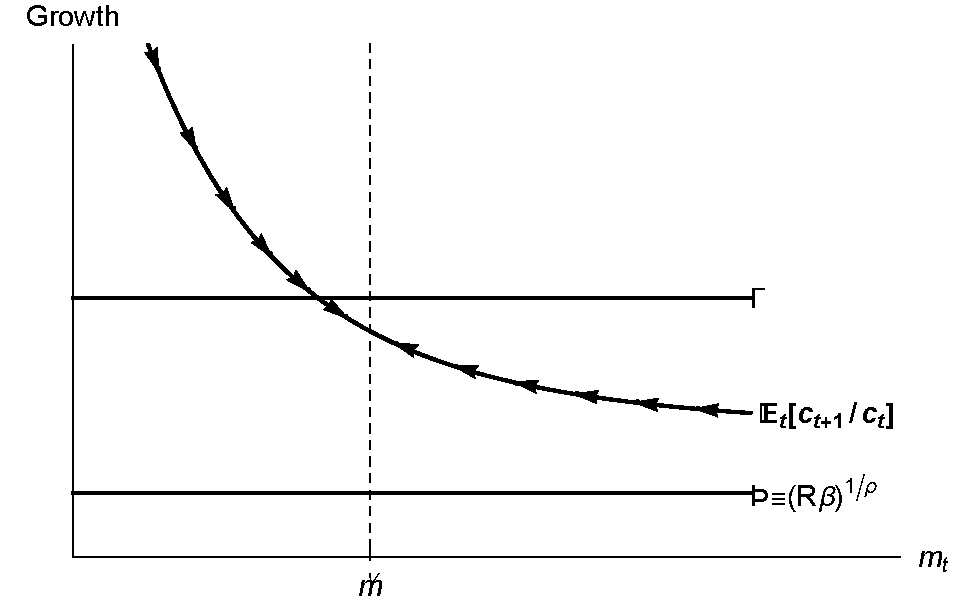
\includegraphics[width=4in]{\FigDir/cGroTargetFig.pdf}}
\end{frame}

\subsection{Bounds On The Consumption Function}
\begin{frame}
\frametitle{Bounds On the Consumption Function}
\centerline{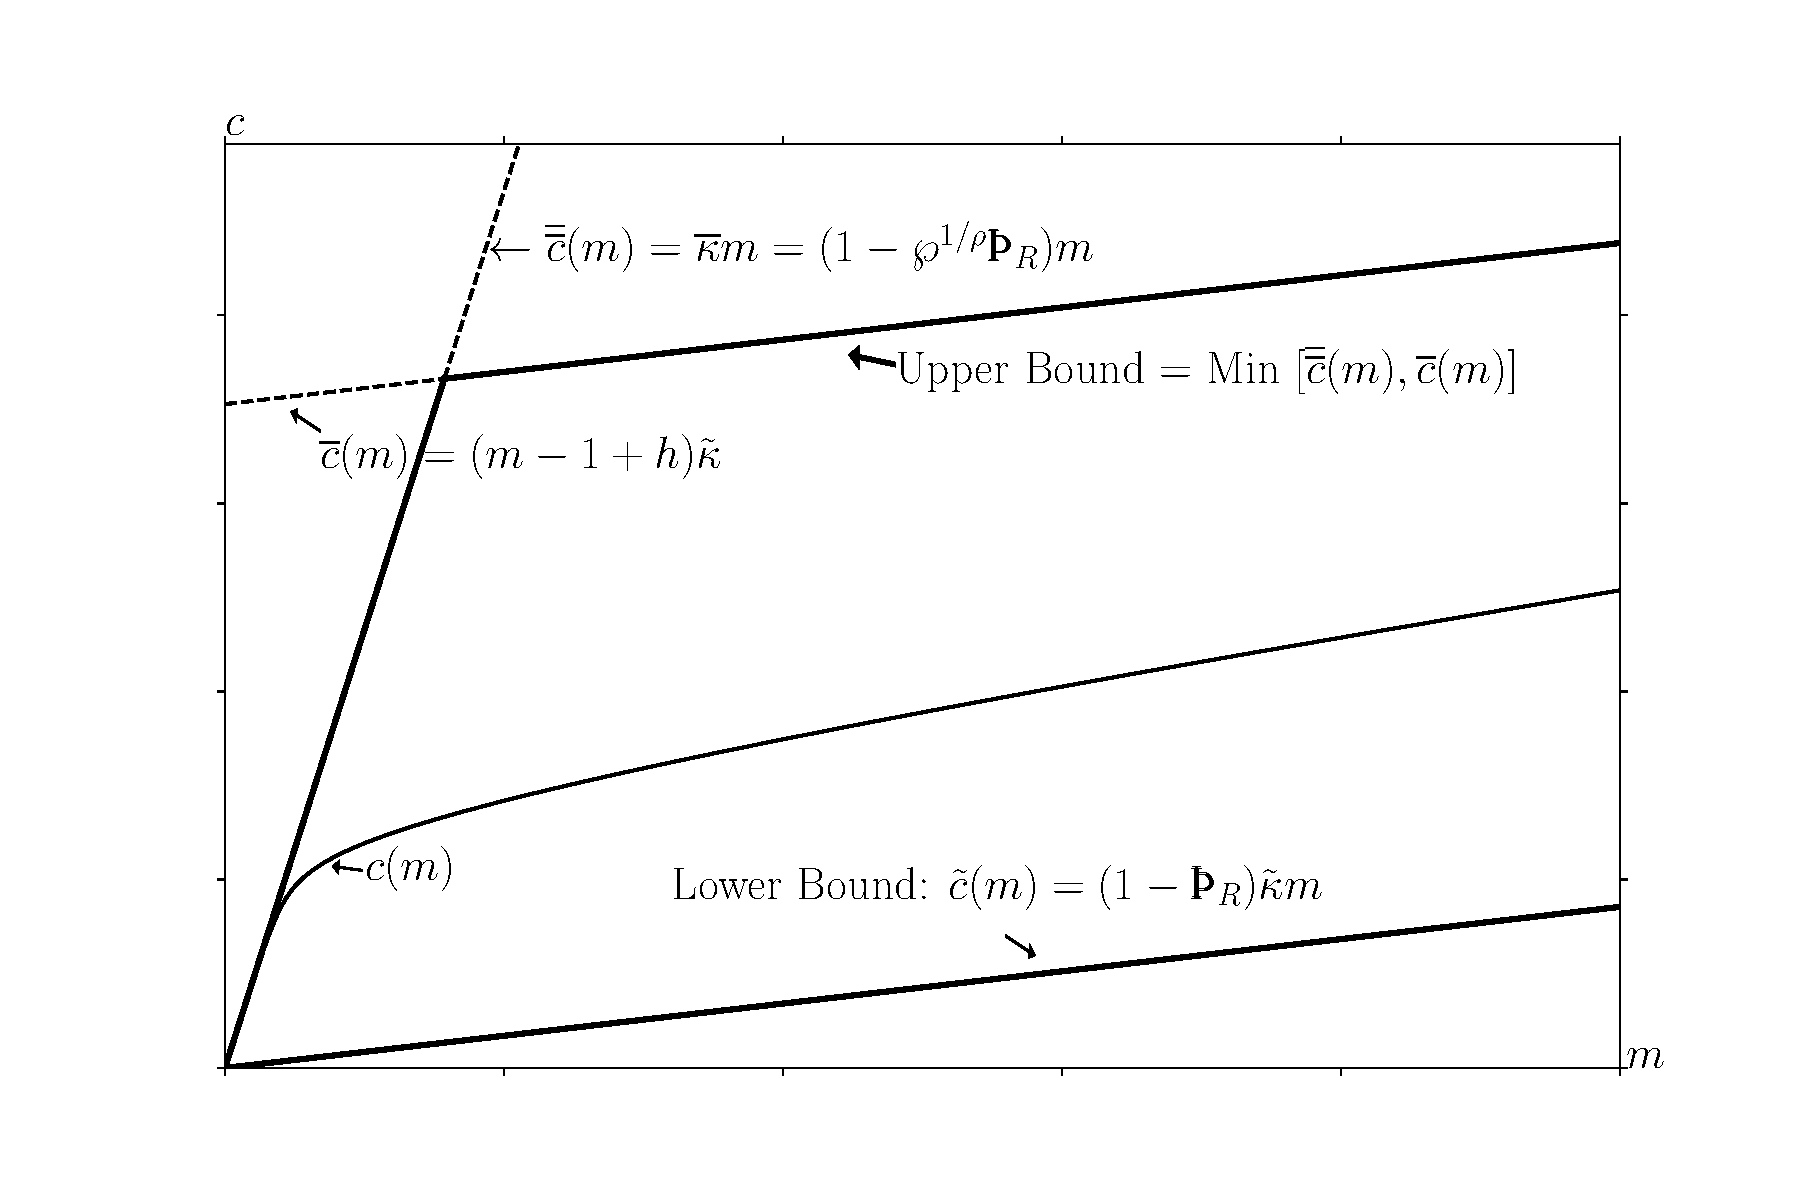
\includegraphics[width=4in]{\FigDir/cFuncBounds.pdf}}
\end{frame}

\begin{frame}
\frametitle{The Marginal Propensity to Consume}
\centerline{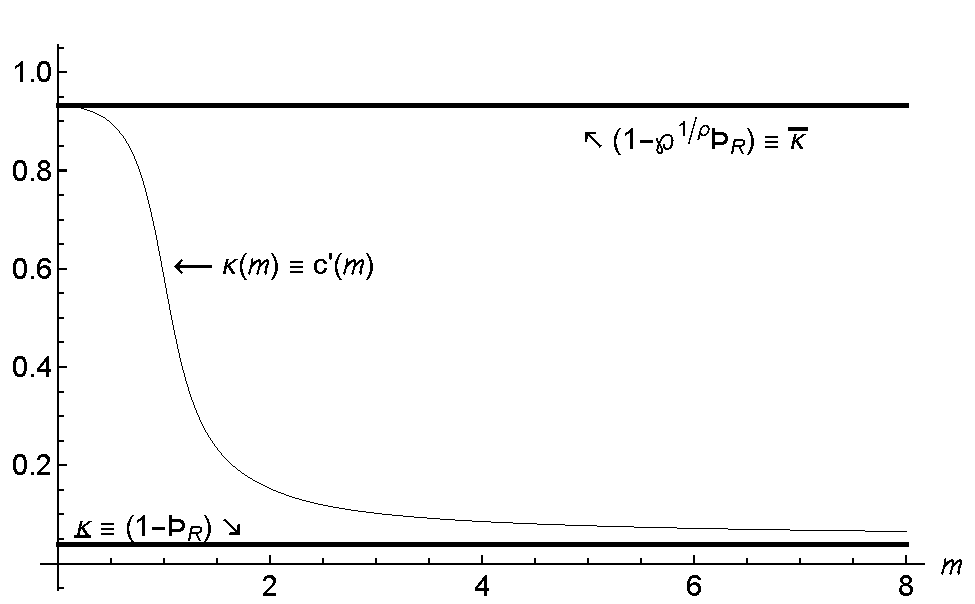
\includegraphics[width=4in]{\FigDir/MPCLimits.pdf}}
\end{frame}

\subsection{The Consumption Function and Target Wealth}
\begin{frame}
\frametitle{The Consumption Function and Target Wealth}
\centerline{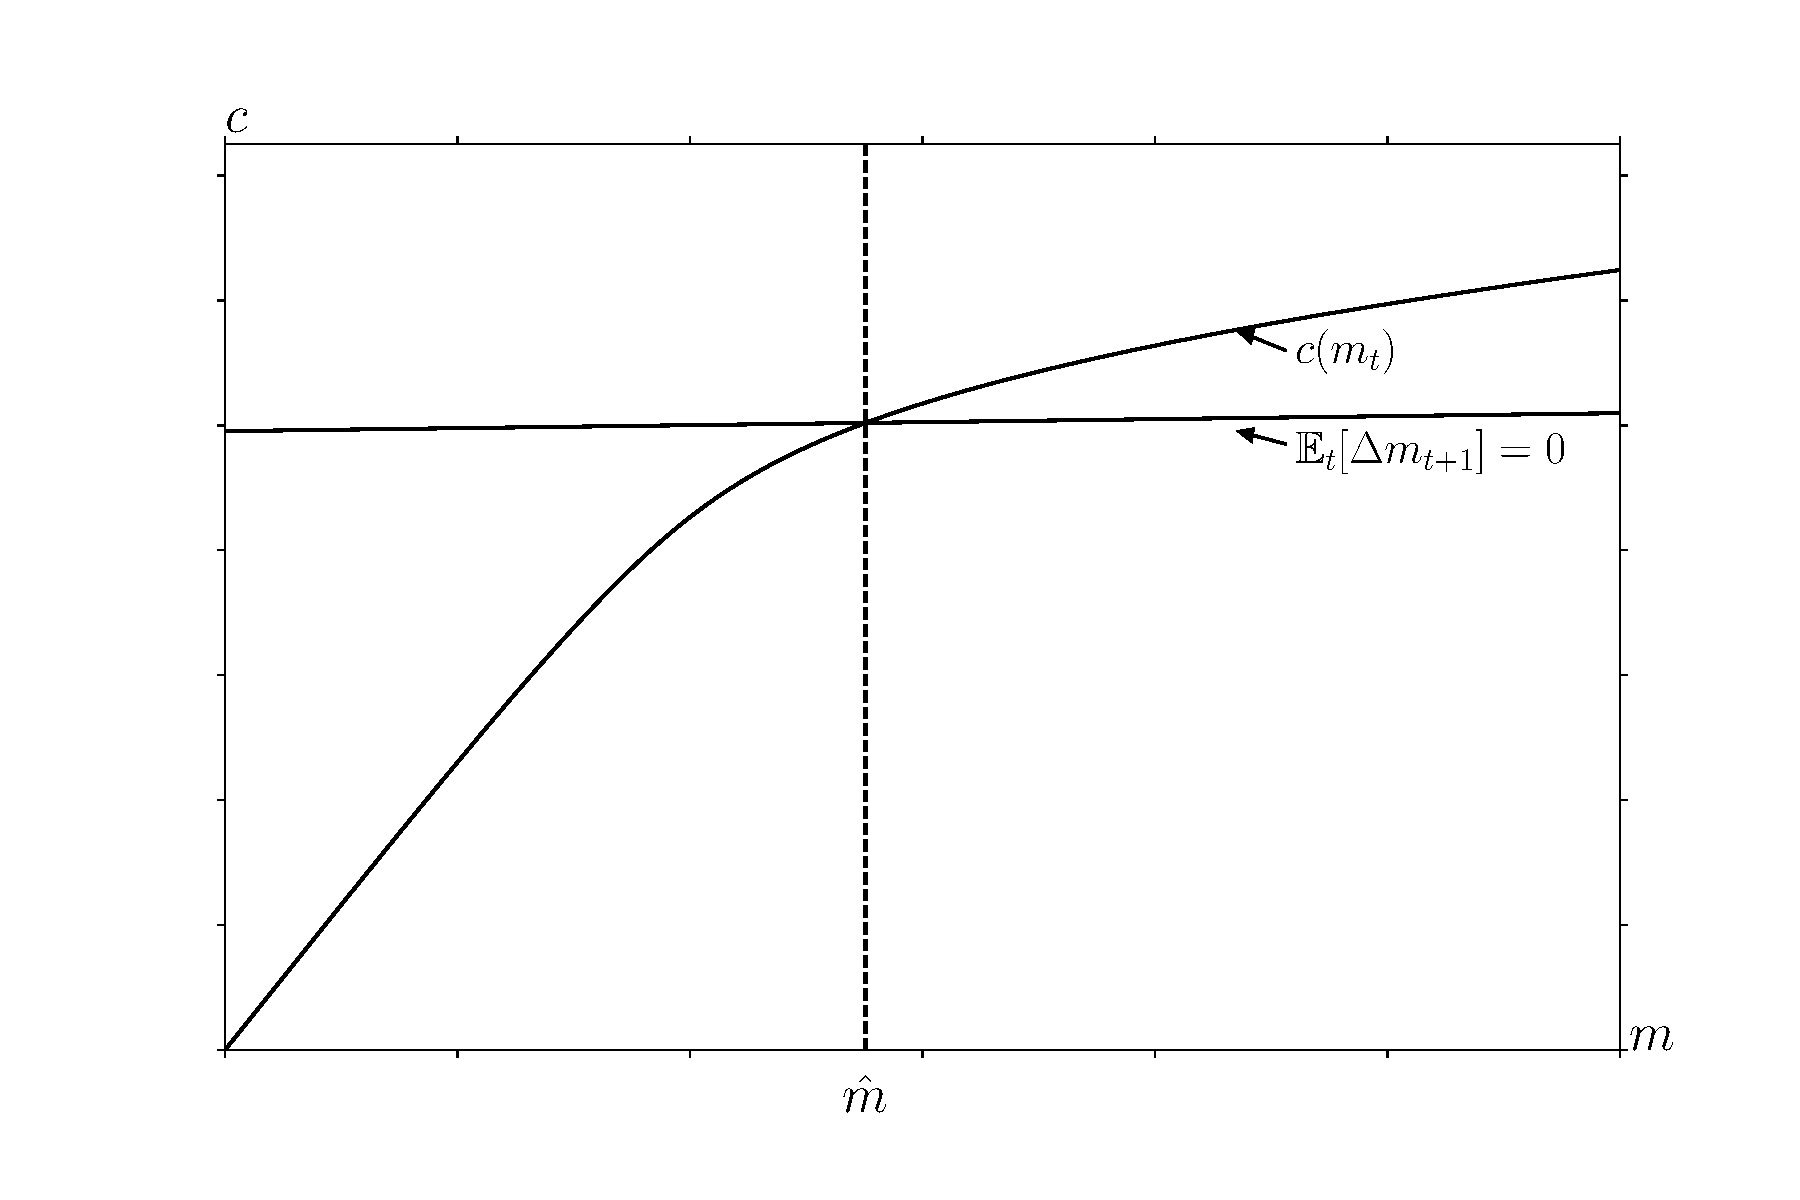
\includegraphics[width=4in]{\FigDir/cRatTargetFig.pdf}}
\end{frame}



\section{A Small Open Buffer Stock Economy}

\subsection{The Invariant Distribution}
\begin{frame}
\frametitle{Convergence To The Invariant Distribution}

\cite{szeidlInvariant} Proves Existence of an Invariant Distribution of 
$\mRat, \cRat, \aRat,$ etc.

\centerline{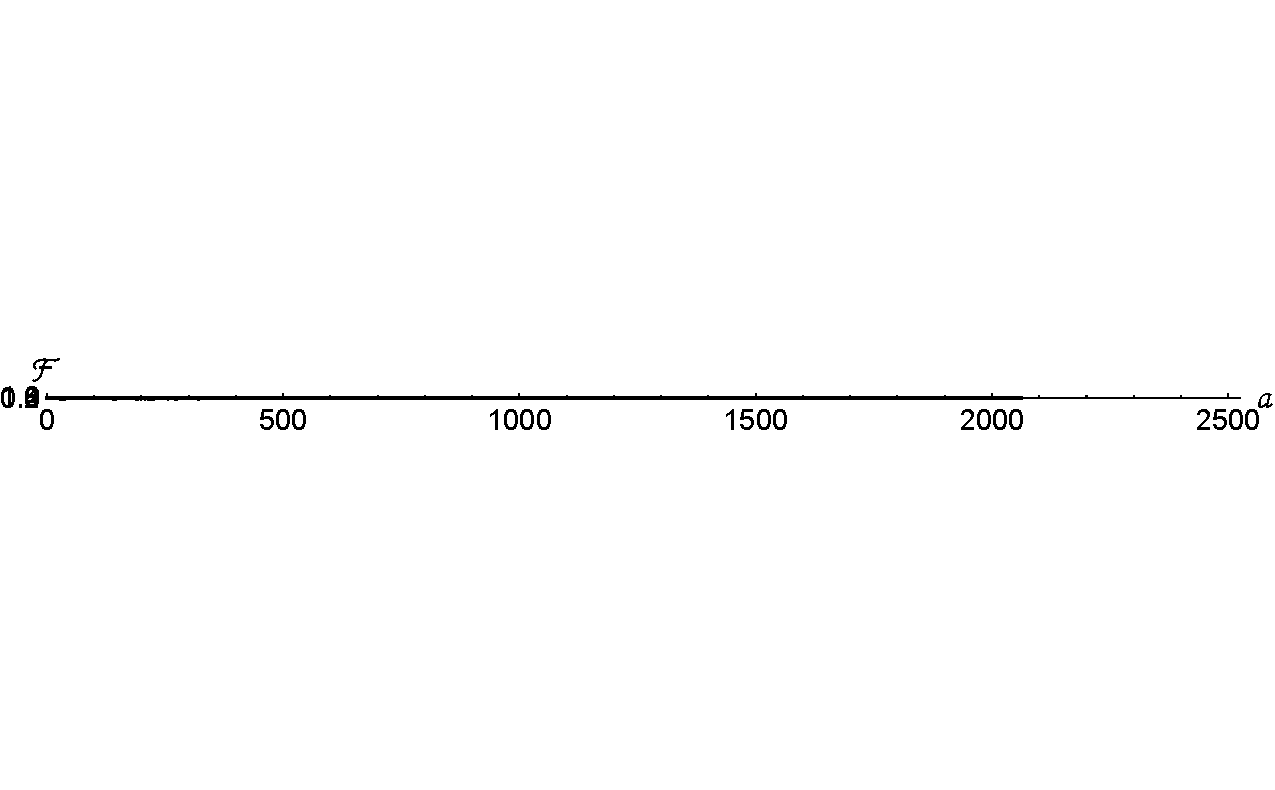
\includegraphics[height=2.5in]{\FigDir/SimCDFsConverge.pdf}}



\end{frame}





\def\newblock{\hskip .11em plus .33em minus .07em}

\begin{frame}

\renewcommand{\bibsection}{\subsubsection*{\bibname }}

\tiny 

\bibliography{\texnameMaster,\econtexBib}

\end{frame}
\end{document}\endinput

% Local Variables:
% eval: (setq TeX-command-list  (remove '("Biber" "biber %s" TeX-run-Biber nil  (plain-tex-mode latex-mode doctex-mode ams-tex-mode texinfo-mode)  :help "Run Biber") TeX-command-list))
% eval: (setq TeX-command-list  (remove '("BibTeX" "%(bibtex) %s" TeX-run-BibTeX nil t                                                                              :help "Run BibTeX") TeX-command-list))
% eval: (setq TeX-command-list  (remove '("BibTeX" "%(bibtex) %s" TeX-run-BibTeX nil (plain-tex-mode latex-mode doctex-mode ams-tex-mode texinfo-mode context-mode) :help "Run BibTeX") TeX-command-list))
% eval: (setq TeX-command-list  (remove '("BibTeX" "%(bibtex) ../LaTeX/%s" TeX-run-BibTeX nil t :help "Run BibTeX")   TeX-command-list))
% eval: (add-to-list 'TeX-command-list	'("BibTeX" "%(bibtex) LaTeX/%s" TeX-run-BibTeX nil t :help "Run BibTeX") t)
% eval: (cond ((string-equal system-type "darwin") (progn (setq TeX-view-program-list '(("Skim" "/Applications/Skim.app/Contents/SharedSupport/displayline -b %n LaTeX/%o %b"))))))
% TeX-PDF-mode: t
% TeX-file-line-error: t
% TeX-debug-warnings: t
% LaTeX-command-style: (("" "%(PDF)%(latex) %(file-line-error) %(extraopts) -output-directory=LaTeX %S%(PDFout)"))
% TeX-source-correlate-mode: t
% TeX-source-correlate-start-server: 0
% TeX-parse-self: t
% End:
